This section outlines the architectural strategy for the flow of the RV8 work cell system, defining the top-level logical view of the design. The system is structured into three distinct layers: Input, Processing, and Output. Each of these layers serves a specific and vital function within the system, enabling the robot to perform dynamic tasks based on the processing of sensor data. This section includes a high-level block diagram that visually illustrates the relationships and interactions between these layers, providing a comprehensive overview of the system's architecture.

\begin{figure}[h!]
	\centering
 	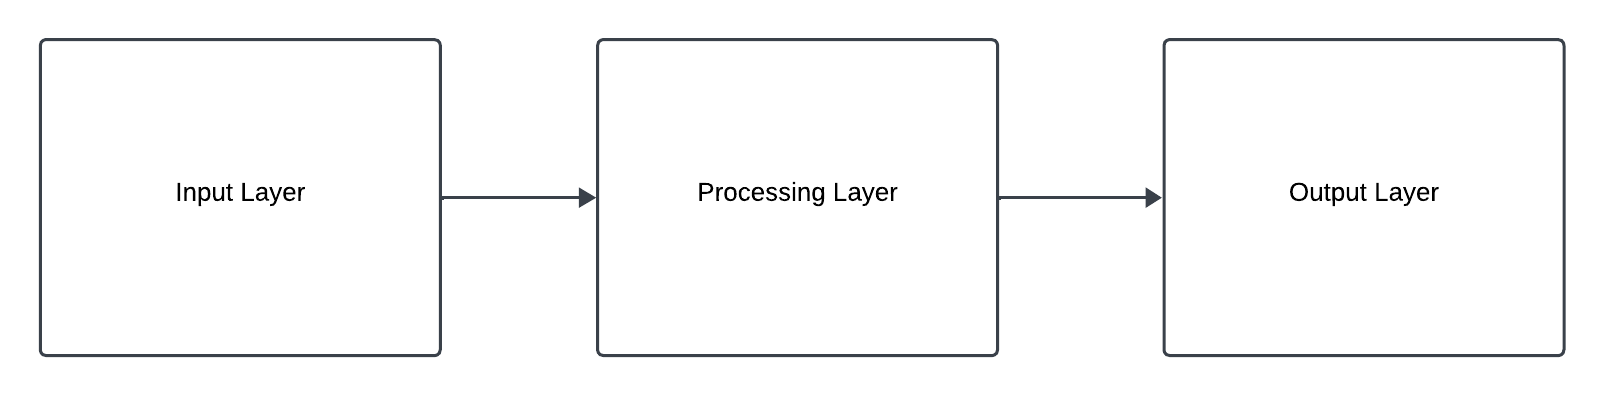
\includegraphics[width=1\textwidth]{images/sys_overview.png}
 \caption{An overview of the higher level layers.}
\end{figure}

\subsection{Input Layer Description}
Since the robot arm will perform tasks as desired by users, this input layer will play an important role in completing these tasks. These sensors gather information from external sources, and based on this information, the internal configuration will be adjusted to respond to different situations. In the input layer, we will have several sensor components, including a QR scanner, a Gate sensor, and E-stops. These sensors will communicate with the processing layer, which primarily controls the robot. The QR scanner reads QR codes and sends the data in digital format to the controller through the Raspberry Pi. The E-stops send a 'True' signal to the controller when any of the E-stops are pressed, causing an immediate system halt, regardless of the ongoing process. Lastly, the Gate sensor determines whether the cage gate is open or closed. When the gate is open, the robot arm will move slowly, as it controls the robot arm's speed and communicates with the controller

\subsection{Processing Layer Description}
Processing layer plays very important role in this product. All the decision making and handling is done in this layer. This layer encompass PLC controller, raspberry pi and a PC. These are interconnected to each other and perform necessary communication to perform given task accurately. PLC controller's primary function is to control robot arm (all joints) and additional axis (in this case a linear rail). Where as, the function of Raspberry pi is to collect data and send it to PC where the decision is made, whether to perform the task on the incoming object (box in this case). PC and PLC talk to each other, in order to align all the joints of the arm and perform task.

\subsection{Output Layer Description}
The output Layer comprises two key components: the robot arm and indicator subsystems, both vital for efficient box palletizing and depalletizing operations. The robot arm, equipped with a gripper, linear rail, and joints, is responsible for handling boxes, creating and removing grips, and configuring its position for tasks. On the other hand, the indicator subsystem employs an industrial light tower to provide visual feedback to operators, signaling different operating modes and safety alerts. These subsystems work in tandem to ensure the smooth execution of tasks within the RV8 work cell system.

